
\chapter{Detector Performance}

The HPS engineering run took place within Hall B at the Thomas Jefferson 
National Accelerator Facility (JLab) in Newport News, VA in the Spring of 2015.
Although the commissioning of the Ecal had already taken place during a run in 
December of 2014, the engineering run would mark the first time that the SVT 
would take on an electron beam and that both subsystems (SVT, Ecal) would be operating in 
conjunction.  Therefore, the performance results from the engineering run were
critical in verifying that all performance metrics were as simulated and to the
planning of future HPS runs.  In the chapter that follows, a review of a few
selected results that demonstrate the performance of both subsystems during the
engineering run will be given.

\section{Performance of the Silicon Vertex Tracker}

Since it was the first time that the SVT would take on physics quality beam, 
care was taken to understand several performance metrics before continuing to
move the SVT towards its final position. 
%In fact, the SVT was ``timed in'' with layers 1-3 position at 4 mm from the beam plane.  
In fact, data was taken with layers 1-3 of the SVT at several positions above the
beam plane and the occupancies were verified
to match what was expected from simulation.  This was of utmost  
importance since the 1\% occupancy requirement at 0.5 mm was crucial to operation of the
SVT. 

All of the data taken with the SVT saw all APV25s configured to their nominal
operating points as listed on Table \ref{}, while all sensors were reverse-biased
to 180 V. All hybrids were being cooled to $\sim$ -14$^{\circ}$C while all FEBs
were being operated at $\sim$ 20$^{\circ}$C.  Finally, only 4 out of the 23,004
SVT channels were found to be dead or noisy.

\subsection{Calibrations}

Preparing the SVT for real physics data-taking required the calibration of the
readout system. This involved the extraction of the baseline 
(pedestal), noise and gain for each of the 23,004 SVT channels.  All 
measurements were made with the APV25s configured to their nominal operating
points and all sensors reverse-biased to 180 V.

The baseline and noise of each of the channels were evaluated by using 
special ``calibration'' runs during which the APV25s were continuously triggered
and read out without any signal present at the input.  The amplitude
of each of the six samples that are 
read out will be Gaussian distributed around the true baseline value with a 
width equal to the noise.  For each of the samples, the baseline distributions
were fit and the baseline and noise extracted (see Figure \ref{fig:baseline_fit}).
\begin{figure}[h!t]
    \centering
    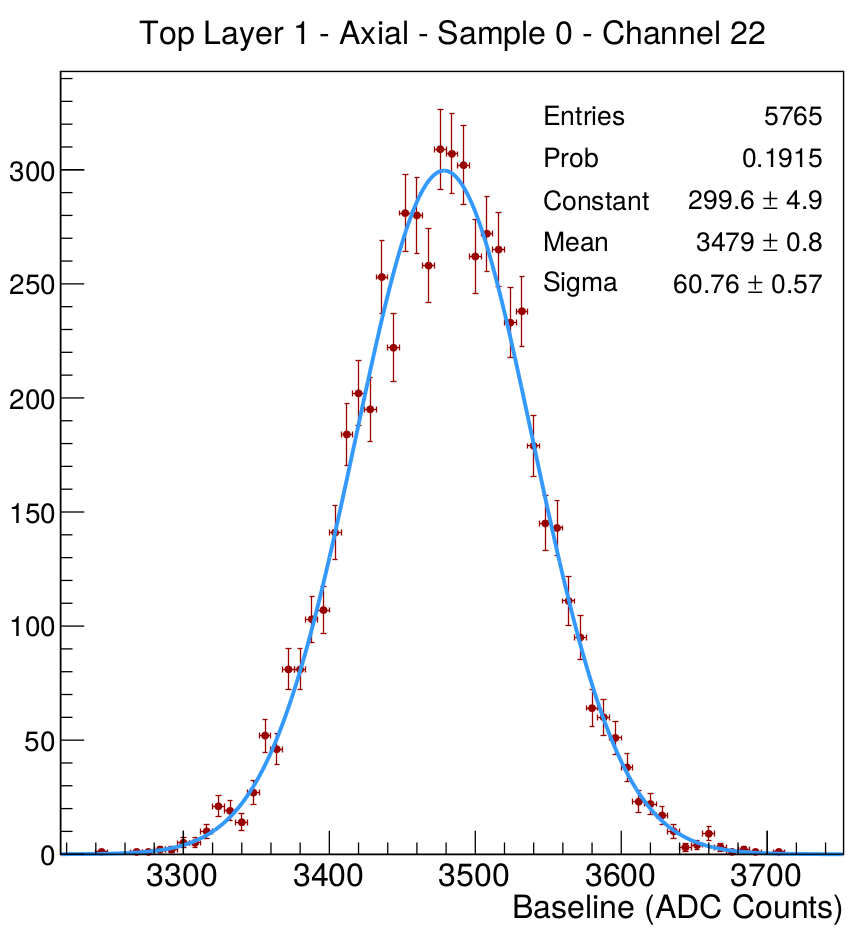
\includegraphics[width=.6\textwidth]{images/baseline_fit_top_l1_axial_sample0_ch22.png}
    \caption{Example illustrating the Gaussian nature of the distribution of
             baseline values.  The distribution is fit with a Gaussian in order 
             to extract the baseline and noise for the channel and sample.}
    \label{fig:baseline_fit}
\end{figure}
A typical distribution of baseline values across a half-module is shown on 
Figure \ref{fig:baseline}.  
\begin{figure}[h!t] 
    \centering
    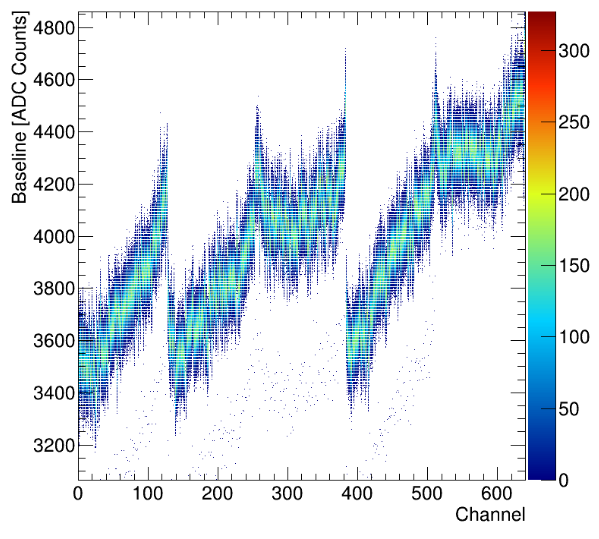
\includegraphics[width=.7\textwidth]{images/baseline.png}
    \caption{Distribution of baseline values across a sensor.}
    \label{fig:baseline}
\end{figure}  
\begin{figure}[h!b]
    \begin{subfigure}{.5\textwidth}
        \centering
        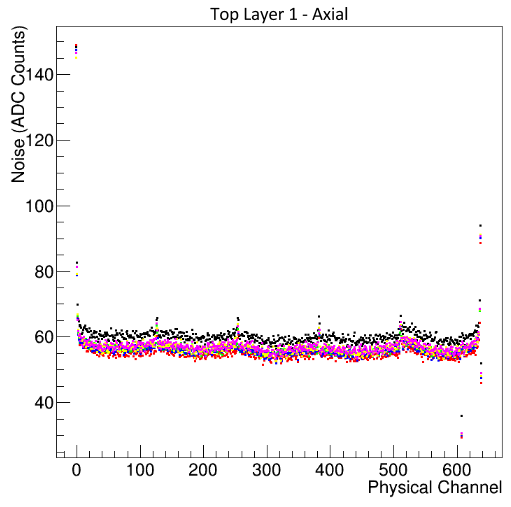
\includegraphics[width=\textwidth]{images/noise_top_layer1_axial.png}
    \end{subfigure}
    \begin{subfigure}{.5\textwidth}
        \centering
        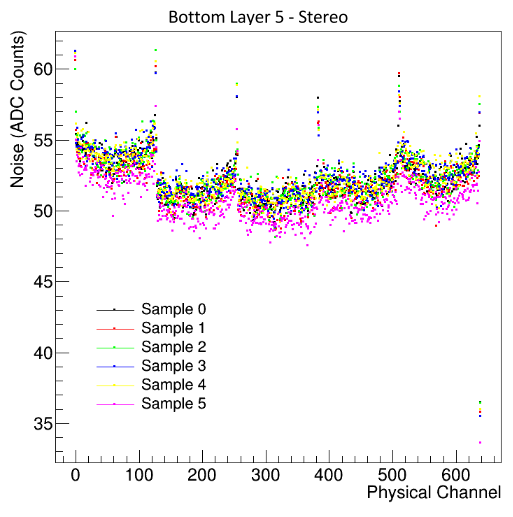
\includegraphics[width=\textwidth]{images/noise_bottom_layer5_stereo.png}
    \end{subfigure}
    \caption{Noise of all channels across a hybrid.}
    \label{fig:noise}
\end{figure}  

Figure \ref{fig:noise} shows the noise across a half-module for each of the 
six samples that are read out.
The noise level of layers 1-3 (4-6) was established
to be between 55-60 (50-55) ADC counts which amounts to $\sim$ 800 - 875 (725 - 800) 
electrons. One thing to note is the large noise values at
the edges of each chip.  This has also been observed by the Compact Muon
Solenoid collaboration
and the cause is still under investigation\footnote{There was an extensive email
discussion with Mark Raymond regarding this issue, but a clear cause was never
pinpointed}. 

The APV25 has a built in calibration circuit that allows for a 
pre-determined signal of known charge to be injected into a subset of channels.
This allows for the accurate determination of the response to a given charge 
via a CR-RC shape fit
to the six pedestal subtracted samples.  The distribution across a hybrid 
of responses to 18,500 electrons is shown on Fig. \ref{fig:response}.
\begin{figure}[h!t]
    \centering
    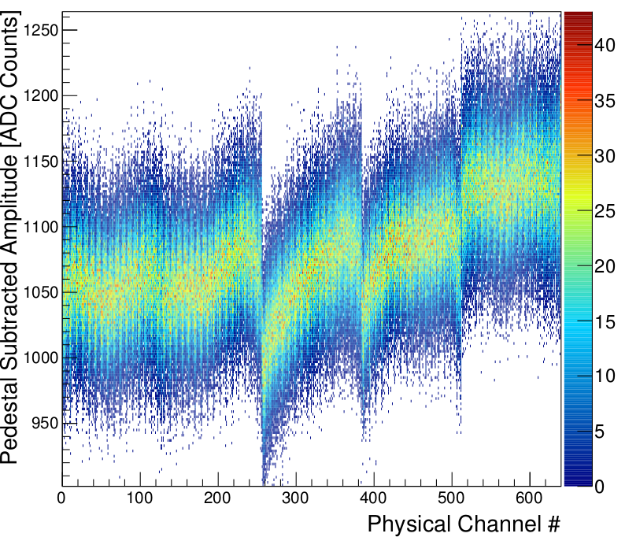
\includegraphics[width=.6\textwidth]{images/response.png}
    \caption{Distribution of responses to 18,500 electrons across one of the 
             half-modules of the Silicon Vertex Tracker.}
    \label{fig:response}
\end{figure}
\begin{figure}[h!b]
    \centering
    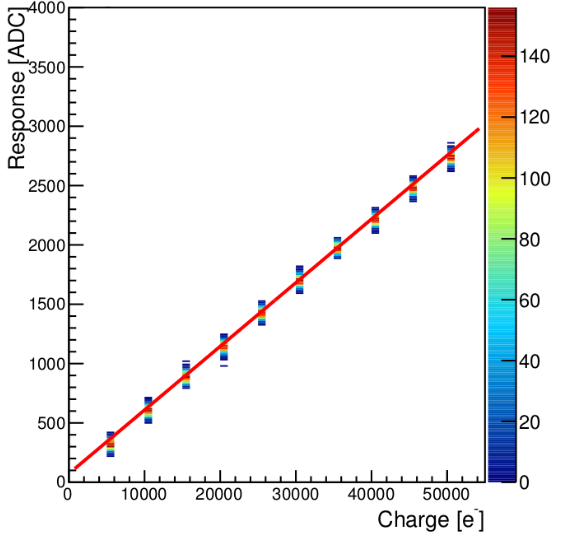
\includegraphics[width=.6\textwidth]{images/response_curve.png}
    \caption{Response curve for a single APV25 channel.}
    \label{fig:response_curve}
\end{figure}
Typically, the response varies by $\sim 7$\% across a half-module. 
The response scale obtained with
the internal calibration circuitry was cross-checked with ionization source
measurements.  

The calibration circuitry was also used to create a response
curve for every channel.  An example of a response curve for one of the 
APV25 channels is shown on Figure \ref{fig:response_curve}.  A linear fit
to the response curve yields the gain and offset of the channel. From the figure, 
it can be seen that the response is approximately linear up to $\sim$ 1 MIP.
This is in agreement with previous measurements which found the gain to be 
linear up to approximately 3 MIPS \cite{French:2001xb}.

\subsection{Occupancy}

When deciding the extent of the ``dead zone'', aside from the radiation field, 
two of the main considerations were the ability to perform robust pattern 
recognition and minimization of pileup within the window of time needed for 
the shaper output to evolve ($\sim$ 250 ns for a 50 ns shaping time).  Using
simulation, it was determined that limiting the occupancy of the strips closest
to the beam within an 8 ns window to less than 1\% fulfilled all of the requirements. 

Since the engineering run marked the first time that the SVT had taken an 
electron beam, care was taken when lowering the first three layers to their 
final position just a mere 15 mrad from the beam.  In fact, the occupancies 
with layers 1-3 at 4, 3, 2, and 1.5 mm away from the beam plane were verified to
match what was predicted from simulation before the SVT was lowered to its final
position.  As can be seen on Figure \ref{fig:occupancies}, once the first
three layers were lowered into their final position (active edge at 0.5 mm away from the
beam plane), the occupancies on the innermost strips were observed to be less
than 1\% as expected.
\begin{figure}[h!b]
    \begin{subfigure}{.5\textwidth}
        \centering
        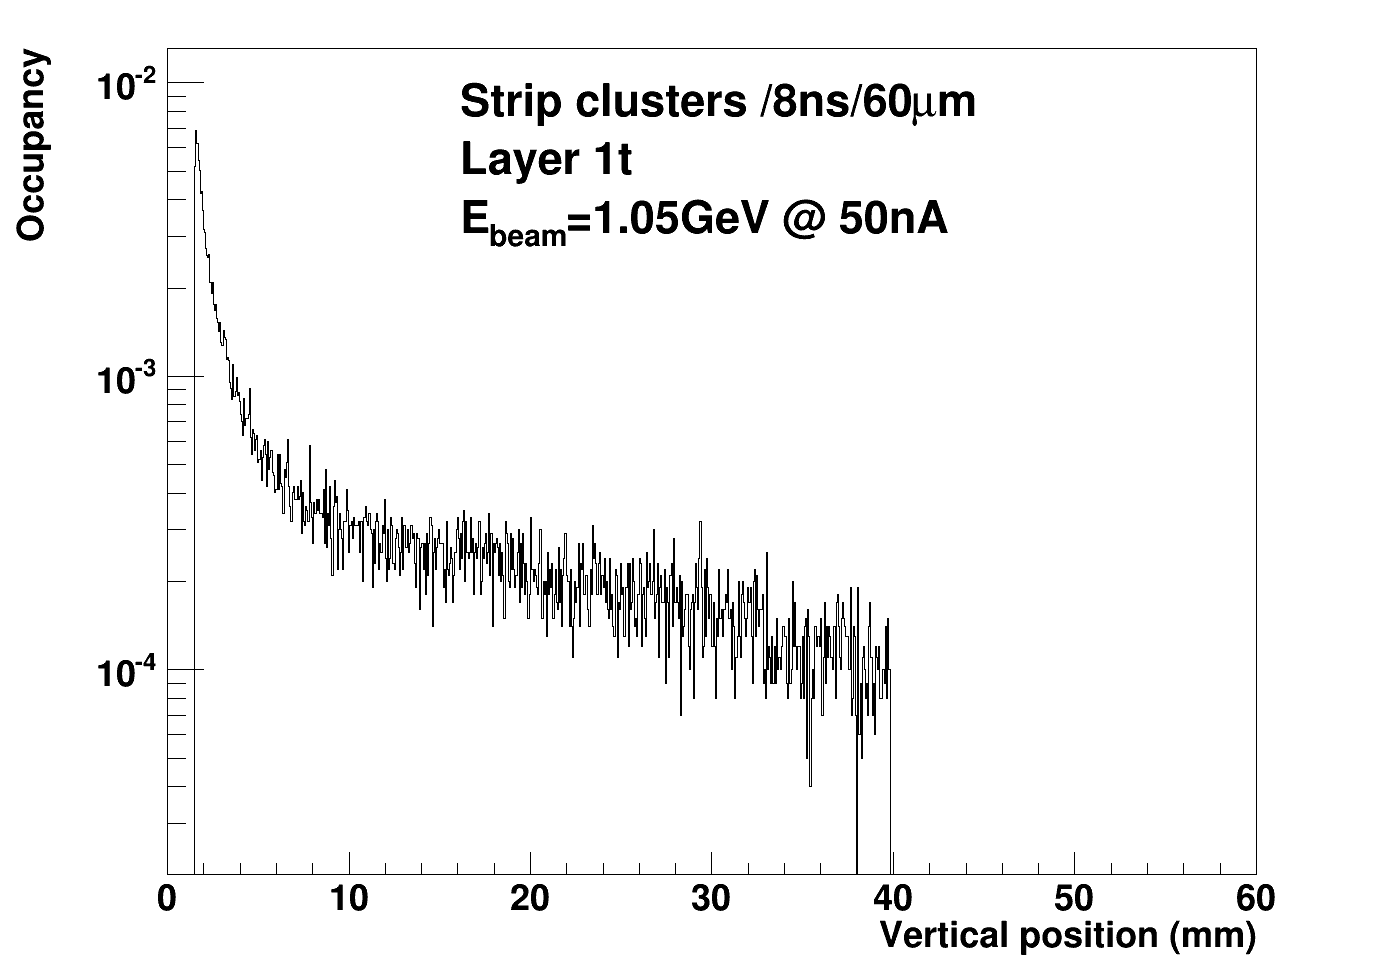
\includegraphics[width=\textwidth]{images/cluster_occupancy_L1t_axial.png}
    \end{subfigure}
    \begin{subfigure}{.5\textwidth}
        \centering
        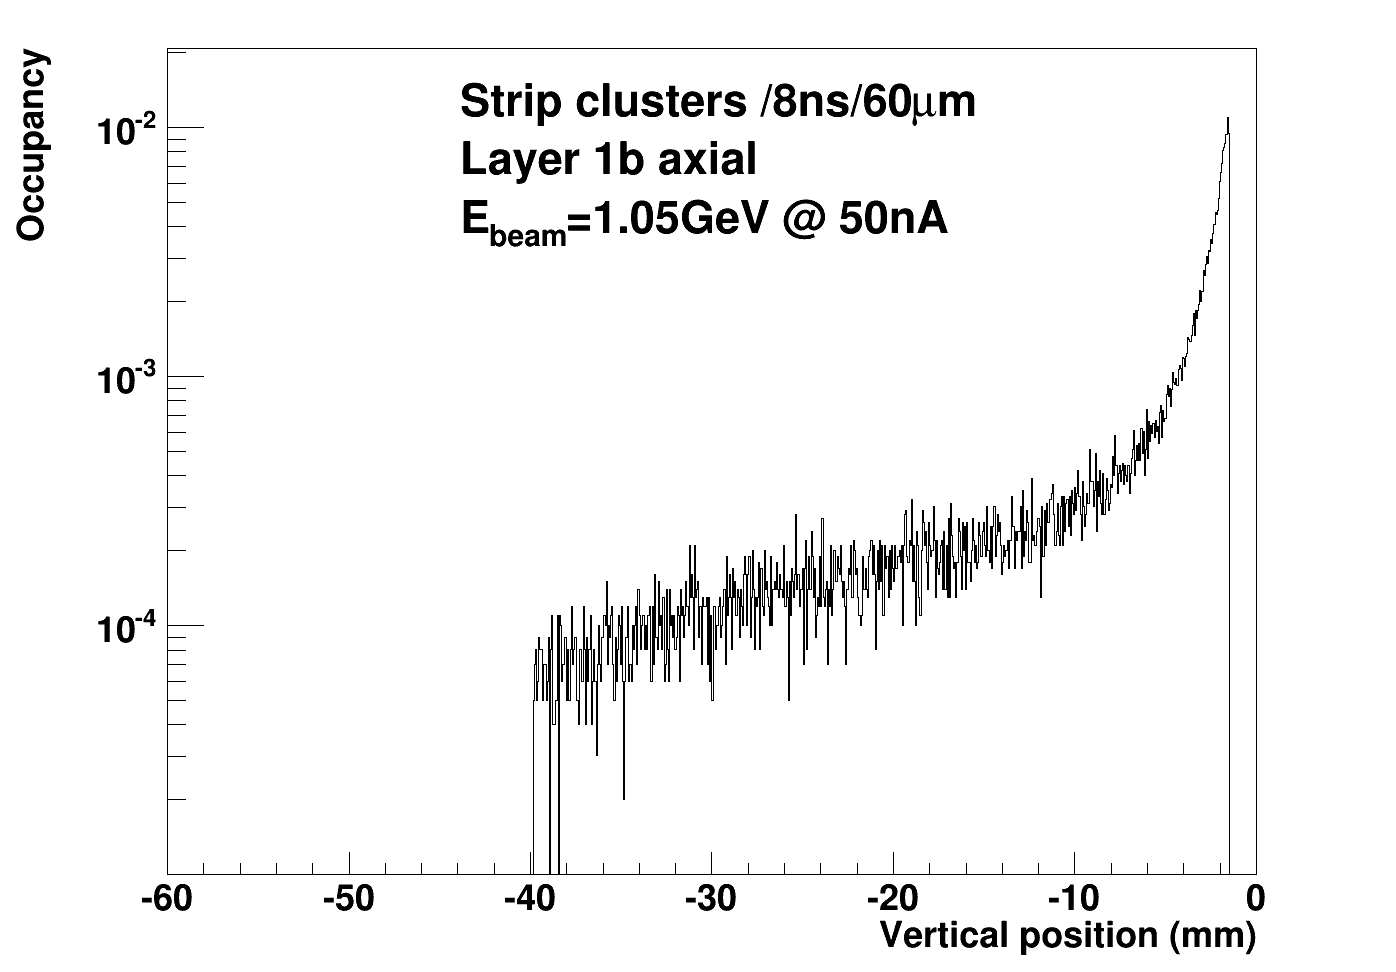
\includegraphics[width=\textwidth]{images/cluster_occupancy_L1b_axial.png}
    \end{subfigure}
    \caption{Occupancies of both top and bottom layer 1.  The occupancies of 
             the innermost strips were observed to be less than 1\% as predicted
             by simulation.}
    \label{fig:occupancies}
\end{figure}  

\subsection{Hit Quality}

When an electron traverses a sensor, the deposited charge may be spread over
several strips.  The signal from each of the strips is processed by the
APV25 and the six samples emerging from each channel are fit using the 
following 3-pole function
\begin{equation}
    f(t) = \frac{\tau_1^2}{(\tau_1 - \tau_2)^3}\left( e^{-\frac{t}{\tau_1}}
            - \sum_{k=0}^2 \left(\frac{\tau_1 - \tau_2}{\tau_1\tau_2}t\right)^k
        \frac{e^{-\frac{t}{\tau_2}}}{k!} \right)
\end{equation}
where $\tau_1$ and $\tau_2$ represent the fall and rise time of the shaper 
signal respectively.  The amplitude and the time of the hit, $t_0$, are then
determined from the fit.

\begin{figure}[h!t]
    \centering
    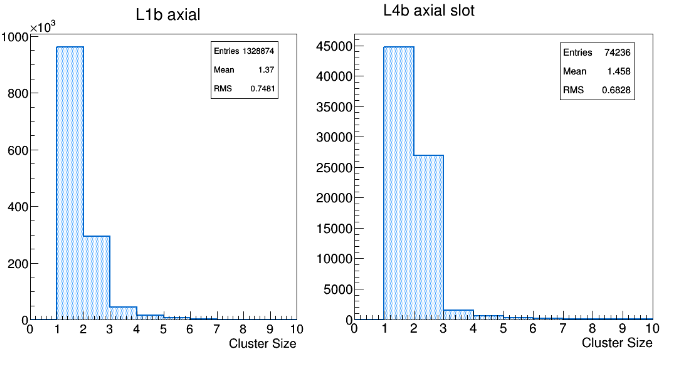
\includegraphics[width=\textwidth]{images/cluster_size.png}
    \caption{The strip multiplicity typically seen during the engineering run.}
    \label{fig:strip_mult}
\end{figure}  
Hits on neighboring strips are clustered using a nearest neighbor
algorithm as follows: 
\begin{itemize}
    \item A list of seeds is created from all raw hits that have a signal-to-noise (S/N)
          $>4$.
    \item Recursively add neighboring strips that have a S/N $>$ 3 until a strip with
          S/N $<$ 3 is found.
      \item Require that neighboring hits have a $t_{0}$ that is within 8 ns of the seed hit.
    \item Repeat the first two steps until seed strips are no longer found.
    \item Require that a cluster has a S/N $>$ 4.
\end{itemize}
The typical strip multiplicity observed during the run is shown on Figure 
\ref{fig:strip_mult}. Figure \ref{fig:cluster_charge} shows the characteristic
\begin{figure}[h!t]
    \centering
    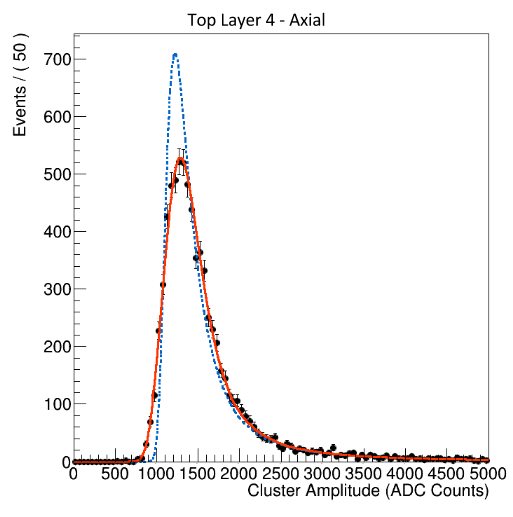
\includegraphics[width=.7\textwidth]{images/top_layer4_axial_cluster_charge.png}
    \caption{Distribution of cluster charge exhibiting the characteristic Landau
             shape.}
    \label{fig:cluster_charge}
\end{figure}  
Landau shape of the cluster charge distribution for one of the sensors.
The cluster charge distribution was then used to measure the S/N to be $\sim$25
which was as expected (See Figure \ref{fig:sig_noise}).
\begin{figure}[h!t]
    \centering
    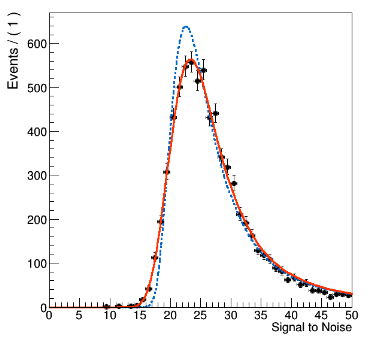
\includegraphics[width=.7\textwidth]{images/sig_noise.png}
    \caption{Example of signal to noise measured during the engineering run.}
    \label{fig:sig_noise}
\end{figure}  

After hits on a sensor have been
clustered, the cluster time is computed as the amplitude-weighted average
of the $t_0$ times from the hits that compose it.  In order to study the hit
time resolution, first a ``track time'' is computed by averaging the cluster 
times of all clusters composing a track.  Then, the residual of each of the 
cluster times is
calculated and the resulting distribution per layer is fit with a Gaussian
to extract the $t_0$ resolution.  The resulting distribution and fit for 
one of the layers in the SVT is shown on Figure \ref{fig:t0_res}.  
\begin{figure}[h!b]
    \centering
    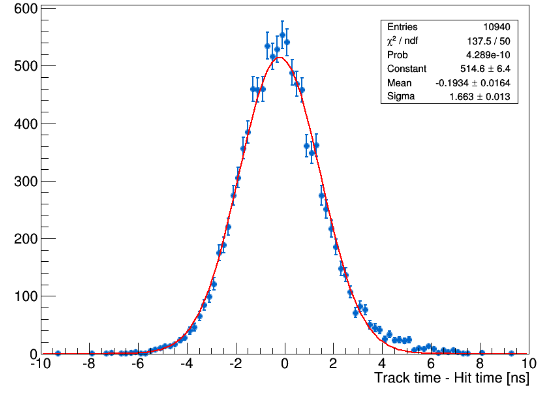
\includegraphics[width=.7\textwidth]{images/t0_res.png}
    \caption{Distribution of cluster time residuals for a single layer of
    the SVT.}
    \label{fig:t0_res}
\end{figure} 
After correcting for offsets, the $t_{0}$ resolution is observed to be $\sim$ 
1.8 ns.

\subsection{Momentum Resolution}

Beam electrons that multiple Coulomb scatter in the target can be used to 
not only verify that the momentum scale is correct but also determine the 
momentum resolution.  These full energy electrons (FEEs) 
were selected by requiring a cluster in the Ecal to have a matching track and
to satisfy the following criteria:
\begin{itemize}
    \item The energy of the cluster of interest in the Ecal  is between 0.8 GeV
          and 1.1 GeV.
    \item The time of the cluster seed relative to the trigger time is between
          39.5 ns and 49.5 ns.
    \item The number of hits composing the cluster has to be greater than 3.
    \item The energy of the cluster seed has to be greater than 400 MeV.
    \item Only consider clusters whose position is above the first row of the 
          Ecal.
\end{itemize}
The momentum distributions of the tracks matched to the clusters that pass the
criteria are shown on Figures \ref{fig:top_p} and \ref{fig:bot_p} split up by volume.  The peaks
of both distributions show that the momentum scale is accurate to within 1\%.  The 
multiple scattering limited momentum resolution of the top (bottom) was measured
to be $\sigma_{p}/p = 6.8\%$ ($\sigma_{p}/p = 7.1\%$) which 
is within 5\% of of the expected value.
\begin{figure}[h!t]
    \centering
    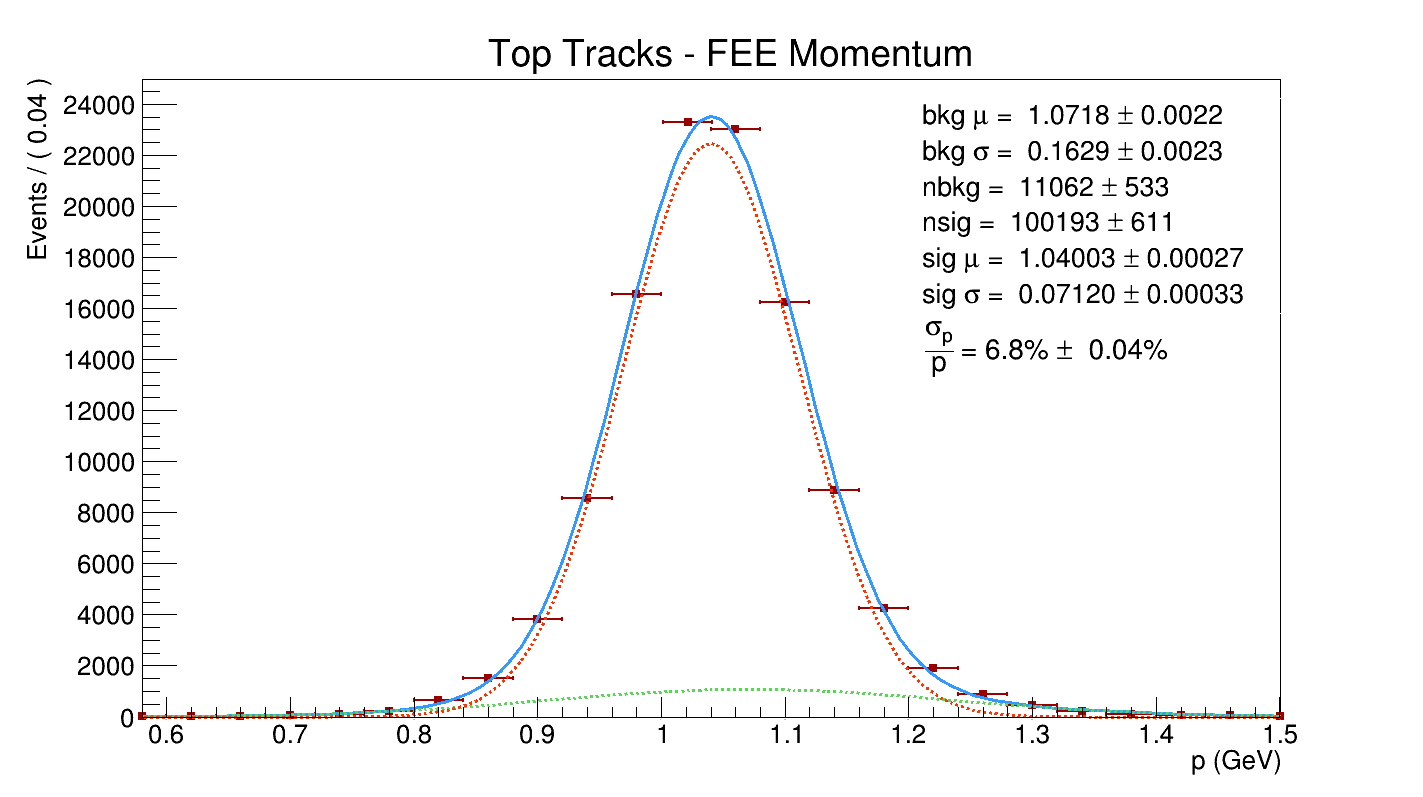
\includegraphics[width=.95\textwidth]{images/20160424_fee_top_tracks_p.png}
    \caption{Top momentum resolution.}
    \label{fig:top_p}
\end{figure}
\begin{figure}[h!b]
    \centering
    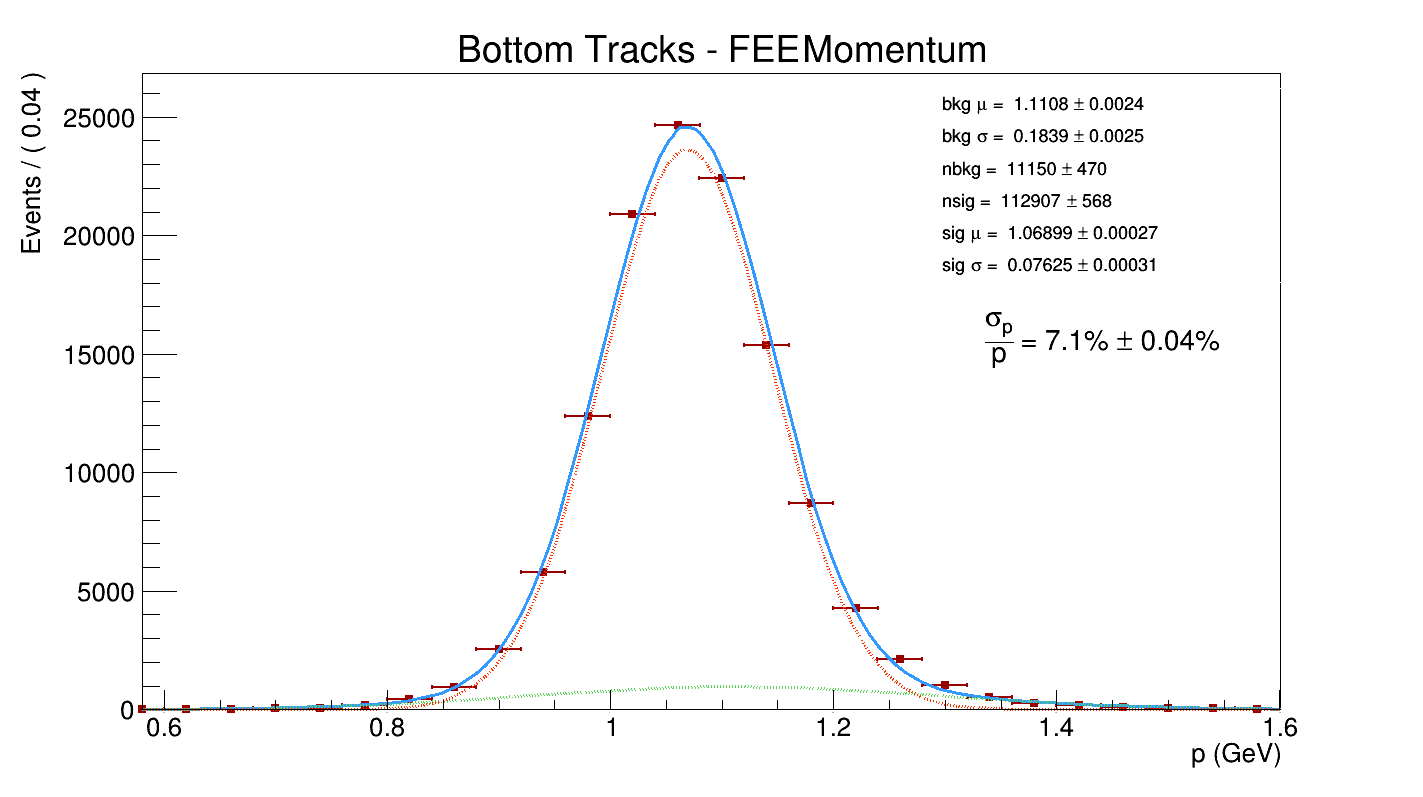
\includegraphics[width=.95\textwidth]{images/20160424_fee_bottom_tracks_p.png}
    \caption{Bottom momentum resolution}
    \label{fig:bot_p}
\end{figure}

\subsection{Tracking Efficiency}

The tracking efficiency was calculated using a tag-and-probe technique.  First
two clusters that are coincident in time are selected in the calorimeter. One
cluster must be on the positron side i.e. $x > 0$ and the other on the electron
side.  The sum of the momentum of the two clusters in required to be greater 
than 0.8 GeV since this is the region of interest for analysis purposes. Then, 
the positron side cluster is required to match to a positron track.  This 
becomes the tag.  The cluster on the electron side is then check to have a 
match to an electron track.  The tracking efficiency is then calculated as 
\begin{equation}
    \varepsilon = \frac{N_{probes}}{N_{tags}}.
\end{equation}
Using this method, the tracking efficiency was found to be $\sim$ 95\%. 

\subsection{Mass resolution}

The heavy photon signal is expected to appear as a Gaussian peak above the QED 
trident invariant mass spectrum with the width corresponding to the mass 
resolution of the experiment.  Thus, determining the mass resolution is a crucial
component of the resonance search, the details of which will be given in Chapter 5.

Determining the mass resolution from data was accomplished by using Moller scatters.
For this particular study, only events which satisfy the ``singles1'' trigger 
requirements were used.  Furthermore, only events where the bias of the SVT was 
on, the SVT was positioned at 0.5 mm from the beam plane and were free of 
data acquisition errors were considered.

Selection of Moller events begins with the requirement that an event have a
a pair of clusters coincident in time satisfying the following criteria:
\begin{itemize}
    \item The two clusters must be coincident within a 1.6 ns window.
    \item The two clusters must be in opposite detector volumes.
    \item The $x$ position of both clusters must be $<0$ i.e. both clusters
          are on the electron side.
\end{itemize}
Once a pair of candidate clusters are found, they are required to match to 
$e^-$ tracks.  Both the tracks are then subjected to the following criteria:
\begin{itemize}
    \item Both tracks are subjected to a $\chi^{2}$ probability cut of 95\%.
    \item The momentum of the tracks are required to be less than 0.7 GeV.
    \item The two electron tracks must come from the same vertex.  In order to
          ensure this, the vertex $\chi^2 <$ 10. The positions along $x$ and $y$
          are then required to lie within an ellipse defined as
          \[
                v_x^2/0.04 + v_y^2/0.0025  = 1.
          \]
\end{itemize}
Finally, the momentum sum of the tracks associated with the clusters must be
greater than 0.8*1.056 GeV and less 1.2 GeV.  The resulting Moller distribution
is shown on Figure \ref{fig:moller_mass}. 

In order to extract the mass resolution, the invariant mass distribution was 
fit with a Crystal Ball function \ref{} plus a Gaussian to account for accidental 
$e^-e^-$ on the low side (See Figure \ref{fig:moller_mass}).  From the 
fit, the mass peak is found to be at 33.2 MeV which is within 3\% of the design
value.  The mass resolution at 33.2 MeV is 1.4 MeV which is within 10\% of what
was predicted by simulation.
\begin{figure}[h!t]
    \centering
    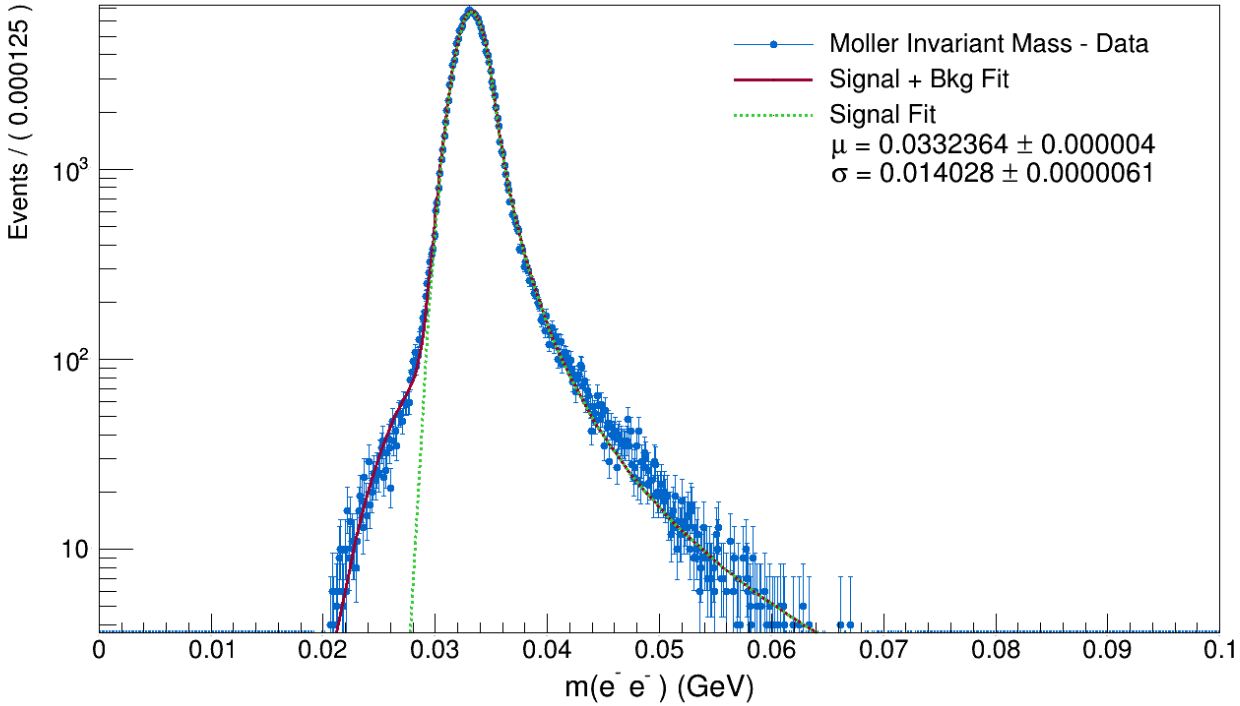
\includegraphics[width=\textwidth]{images/moller_invariant_mass.png}
    \caption{Moller invariant mass distribution.}
    \label{fig:moller_mass}
\end{figure}

Determining the mass resolution as a function of mass was done by using $A'$ 
signal and Moller Monte Carlo. The resulting mass resolutions at each mass 
hypothesis are shown on Figure \ref{fig:mass_resolution}. 
\begin{figure}[h!t]
    \centering
    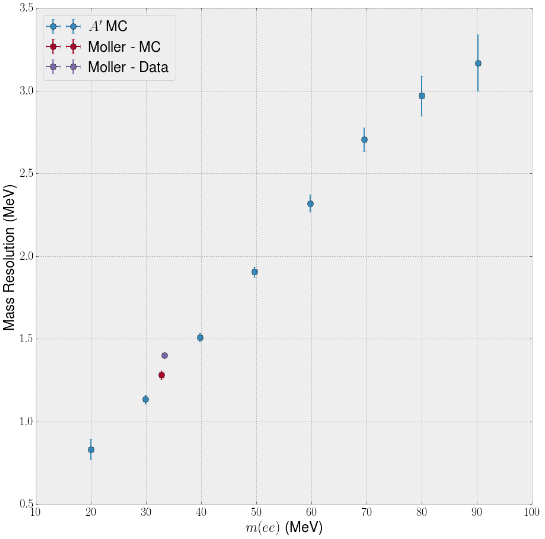
\includegraphics[width=.8\textwidth]{images/invariant_mass_curve.png}
    \caption{Mass resolution as a function of mass.}
    \label{fig:mass_resolution}
\end{figure}
The mass resolution as a function of mass was found to be best modeled using
a third order polynomial of the form
\begin{equation}
    \sigma_{m}(m_{ee}) = -6.166 x^3 + 0.9069 x^2 - 0.00297 x + 0.000579
\end{equation}
This equation was used in the resonance search described in Chapter 5. 

%\section{Performance of the Electromagnetic Calorimeter}

\section{Trigger Performance}

The performance of the trigger was studied by using a simulation of the trigger
and comparing it to the hardware trigger.  First, the raw FADC hits are converted
to GTP clusters using a simulation of the hardware clustering algorithm. Then
a simulation of the trigger decision was compared to the actual decision reported
by the hardware trigger.  The results of the study are listed on Table 
\ref{tab:trig_eff}.
\begin{table}[h!]
    \centering
    \begin{tabular}{lc}
        \toprule
        \textbf{Trigger Type} & \textbf{Efficiency} \\
        \midrule
        \midrule
        Singles               & 99.6\%              \\
        Pair                  & 99.7\%              \\
        \bottomrule
    \end{tabular}
    \caption{Trigger efficiency of both Singles and Pair triggers.}
    \label{tab:trig_eff}
\end{table}



